\documentclass[class=report, crop=false, 12pt,a4paper]{standalone}
\usepackage{enumitem}
\usepackage{multicol}
\usepackage{etoolbox}
\AtBeginEnvironment{quote}{\singlespacing\small}
\usepackage{setspace}
\onehalfspacing
\usepackage{graphicx}
\usepackage{float}
\usepackage{siunitx}
\sisetup{detect-all}
\begin{document}
\section{Second Law of Thermodynamics}
First, let us remind ourselves of the first law of thermodynamics and some of its limitations. 
\begin{quote}
  \begin{center}
    Energy can neither be created or destroyed during a process; it can only change forms.
  \end{center}
\end{quote}
\begin{itemize}[noitemsep]
  \item A certain energy balance will hold when a system undergoes change or a thermodynamic process.
  \begin{itemize}
    \item But does not give information on whether the change of state or the process is at all feasible or not.
  \end{itemize}
  \item It cannot indicate whether a metallic bar of uniform temperature can spontaneously become warmer at one end and cooler at the other.
  \begin{itemize}
    \item However, if that process did occur, all that law can state is that the energy gained at one end would exactly equal the energy lost at the other.
  \end{itemize}
\end{itemize}
The second law of thermodynamics provides the criterion as to the \emph{probability} of various processes. Spontaneous processes in nature occur only in one direction. Heat flows from a body at high temperature to a body at low temperature; water always flows downwards etc. The spontaneity of the process is due to finite driving potential, sometimes called 'force' or 'cause', e.g. a temperature or concentration gradient or an electric potential. What happens as a result of this finite driving potential is called the 'flux' or the 'current' or the 'effect' (heat transfer, mass transfer, flow of electric current). This directional law puts a limitation on energy transformation other than that imposed by the first law. 

There is also a qualitative difference between heat and work. Energy supplied as work can be completely converted to heat, e.g. paddle wheel work on a liquid in an adiabatic vessel. However, the complete conversion of heat into work is not possible, thus making heat and work not completely interchangeable forms of energy. Also, we considered the problem of a simple steam power plant and by using the Steady Flow Energy Equation (i.e. first law) and the properties of steam were able to calculate the work done and heat transfers for individual components. However, we are not yet able to understand ways of improving steam engine efficiency.

The second law is based on experimental observation and was the result of the question, 'how efficient can one make a steam engine?' From now we will start by considering engines and define them with the precision that thermodynamics requires. The sort of steam engines we shall discuss are heat devices in boxes with no fluid entering or leaving but with just heat and work crossing the boundaries.
\subsection{Heat engine}
Definition:
\begin{quote}
  \begin{center}
    A heat engine (or Cyclic Heat Power Plant - CHPP) is a continously operating thermodynamic system at the boundary of which there are heat and work transfers.
  \end{center}
\end{quote}
Notes:
\begin{itemize}[noitemsep]
  \item 'Continously operating' means that the state of the system exhibits only periodic (cyclic) changes.
  \item The heat engine is a thermodynamic system and so no matter crosses the boundary e.g. simple steam power plant and closed-cycle gas turbine plant.
\end{itemize}
\newpage
\begin{figure}[H]
  \begin{center}
    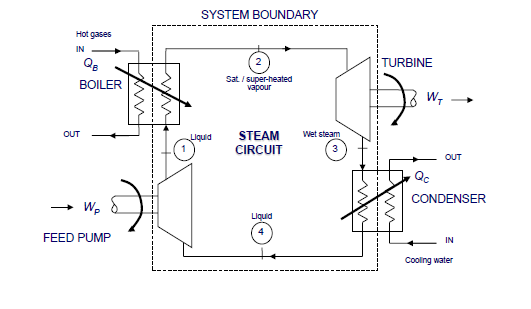
\includegraphics[width = \textwidth]{../img/SimpleSteamPP}
    \caption{A simple steam power plant}
  \end{center}
\end{figure}
\begin{figure}[H]
  \begin{center}
    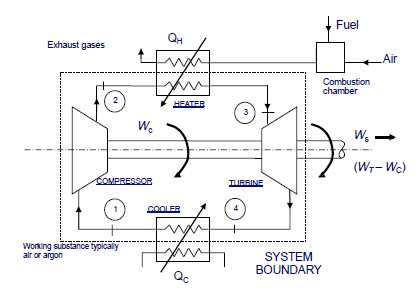
\includegraphics[width = \textwidth]{../img/ClosedCycleGasPP}
    \caption{A closed cycle gas power plant}
  \end{center}
\end{figure}
\begin{figure}[H]
  \begin{center}
    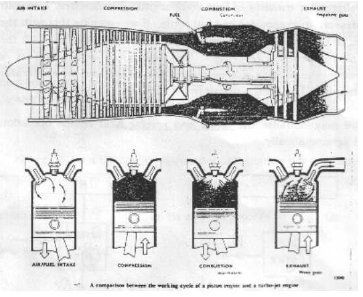
\includegraphics[width = \textwidth]{../img/DieselEngine}
    \caption{A diesel engine}
  \end{center}
\end{figure}

Diesel engines (and internal combustion engines generally) are not heat engines (CHPP) because matter crosses its boundaries. A jet engine is also not a CHPP because matter, air, fuel and exhaust cross the boundary of the system.
\subsection{Reversed heat engine}
The definition of a heat engine says nothing about the direction of heat and work transfers. Thus, this makes a domestic refrigerator a heat engine. The domestic refrigerator consists of: 
\begin{multicols}{2}
  \begin{itemize}[noitemsep]
    \item Condenser.
    \item Vapour compressor.
    \item Evaporator.
    \item Throttle.
  \end{itemize}
\end{multicols}
Compare this to other heat engines e.g. steam/gas turbine power plants, where the component roles are reversed.
\begin{multicols}{2}
  \begin{itemize}[noitemsep]
    \item Boiler $>$ Condenser.
    \item Turbine $>$ Compressor.
    \item Condenser $>$ Evaporator.
    \item Pump $>$ Throttle.
  \end{itemize}
\end{multicols}
\section{Reversibility}
\section{Entropy}
\end{document}